%% Based on the official fithesis4 example for the Faculty of Informatics,
%% Masaryk University: https://www.fi.muni.cz/tech/unix/tex/fithesis.html
\documentclass[
  digital,     %% Replace with `printed` for the printed version.
  oneside,     %% Replace with `twoside` if you also plan to print
               %% double-sided (use at least 120 g/m² paper).
  nosansbold,  %% Replace with `sansbold` for sans-serif bold text.
  nocolorbold, %% Replace with `colorbold` for blue bold text.
  lof,         %% Replace with `nolof` to hide the List of Figures.
  lot,         %% Replace with `nolot` to hide the List of Tables.
]{fithesis4}

%% Locales
\usepackage[resetfonts]{cmap}
\usepackage[T1]{fontenc}
\usepackage[main=english]{babel}   
           

%% Thesis metadata
\thesissetup{
    date        = \the\year/\the\month/\the\day,
    university  = mu,
    faculty     = fi,
    type        = bc,  %% bc = bachelor, mgr = master, rig, phd
    department  = Faculty of Informatics,
    author      = Michal Bahna,
    gender      = m,   %% m or f; affects Czech/Slovak declension
    advisor     = Milan Brož,
    title       = OpenSSL certificates analysis using sec-certs,
    TeXtitle    = OpenSSL certificates analysis using sec-certs,
    keywords    = {keyword1, keyword2, ...},
    TeXkeywords = {keyword1, keyword2, \ldots},
    abstract    = {%
      This is the abstract of my thesis, not yet there.
      Please keep in mind, the bibliography is not yet there, there are only links for my internal use
    },
    thanks      = {%
      These are the acknowledgements for my thesis.
    },
    bib         = references.bib,
    %% Remove the following line to use the JVS 2018 faculty logo.
    facultyLogo = fithesis-fi,
    %% Uncomment and replace with the filename of your scanned
    %% thesis assignment.
%%    assignment  = assignment.pdf,
}

%% Additional packages
\usepackage{paralist} %% Compact list environments
\usepackage{amsmath}  %% Mathematics
\usepackage{amsthm}
\usepackage{amsfonts}
\usepackage{url}      %% Hyperlinks
\usepackage{booktabs} %% Table rules
\usepackage{listings} %% Source code highlighting
\lstset{
  basicstyle      = \ttfamily,
  identifierstyle = \color{black},
  keywordstyle    = \color{blue},
  stringstyle     = \color{teal},
  commentstyle    = \itshape\color{magenta},
  breaklines      = true,
}
\usepackage{floatrow} %% Putting captions above tables
\floatsetup[table]{capposition=top}
\usepackage[babel]{csquotes} %% Context-sensitive quotation marks
\usepackage{graphicx} %% Images
\graphicspath{{figures/}}

\theoremstyle{definition}
\newtheorem{definition}{Definition}[chapter]

\begin{document}

%% The introduction is unnumbered by FI convention, so the heading and
%% table of contents entry are added manually.
\chapter*{Introduction}
\markright{\textsc{Introduction}}
\addcontentsline{toc}{chapter}{Introduction}

Security certifications are how buyers of IT products, particularly
in the public sector, are given assurance that a product meets a defined
set of security requirements. The two schemes studied in this thesis are
Common Criteria (CC)~\cite{iso15408}, which evaluates IT products
against a stated set of security claims, and FIPS~140~\cite{fips1402,fips1403},
which validates cryptographic modules. Both produce public documents, and
both describe products that are rarely built from scratch: cryptography
in particular tends to come from a small number of shared libraries.

OpenSSL is one of the most prominent of these libraries. The effects of
its widespread reuse became visible in 2014, when the Heartbleed
vulnerability (CVE-2014-0160) prompted large-scale measurement of how
many services were exposed and how quickly they were
patched~\cite{durumeric2014heartbleed}. In the same year, LibreSSL was
forked from OpenSSL~\cite{libressl} and Google announced
BoringSSL~\cite{langley2014boringssl}. Today, the library that a product
calls ``OpenSSL'' may be one of several related code bases.

\section*{Problem statement}

Certification documents are not designed to answer supply-chain questions.
Which third-party cryptographic library a product uses, and in which
version, is usually disclosed, if at all, in the prose of a PDF
document. The sec-certs project~\cite{janovsky2024seccerts} has made
thousands of these documents accessible and machine-readable, but tracing
the lineage of one specific library across Security Targets, certification
reports, and maintenance reports still requires a targeted analytical
pipeline. As a result, it is difficult to establish how far OpenSSL and
its forks have spread through certified products, or how far certified
products trail the upstream releases they depend on.

\section*{Goals and research questions}

This thesis investigates the footprint, usage patterns, and lifecycle of
OpenSSL and its forks in the certified products indexed by sec-certs.org,
and implements an extensible, reproducible framework for analyzing and
visualizing these dependencies. It addresses three research questions:

\begin{description}
  \item[RQ1] How widely are OpenSSL and its clones and forks represented
    across Common Criteria and FIPS~140 certifications indexed by
    sec-certs.org?
  \item[RQ2] What is the gap between upstream OpenSSL releases and the
    validation or re-validation of dependent certified products?
  \item[RQ3] How can automated data mining, AI/NLP document parsing, and
    interactive visual tooling be integrated into sec-certs workflows to
    reliably track cryptographic dependencies and produce reproducible
    business intelligence?
\end{description}

The thesis is an empirical study of public certification data. Manual
reverse engineering, side-channel analysis, and binary-level vulnerability
research of certified products are out of scope, as are certification
frameworks other than CC and FIPS~140.

\section*{Contributions}

The thesis makes two contributions:

\begin{itemize}
  \item an empirical analysis of vendor adoption trends, re-certification
    patterns, and compliance lag in open-source cryptography; and
  \item an open toolkit of Jupyter notebooks and processing scripts that
    extends sec-certs and supports ongoing monitoring and reproducible
    analysis.
\end{itemize}

\section*{Thesis outline}

Chapter~\ref{ch:background} introduces the certification schemes, the
OpenSSL family of libraries, the sec-certs project, and related work.
Chapter~\ref{ch:method} defines the dataset, the detection heuristics, the
AI-assisted parsing, and the metrics. Chapter~\ref{ch:results} presents the
findings for each research question, and Chapter~\ref{ch:discussion}
interprets them and considers threats to validity. The Conclusion summarizes
the contributions and proposes future work.

\chapter{Background}
\label{ch:background}

This chapter introduces the two certification schemes, the family of
libraries under study, and the sec-certs project, and then reviews related
work.

\section{Common Criteria}
\label{sec:cc}

Common Criteria, standardized as ISO/IEC~15408~\cite{iso15408}, is a
framework for evaluating the security of IT products. The product under
evaluation is called the Target of Evaluation (TOE). The vendor describes
the TOE and its security claims in a Security Target (ST), which may claim
conformance to a Protection Profile, a reusable set of requirements for a
class of products. An accredited laboratory evaluates the TOE against those
claims at a chosen Evaluation Assurance Level (EAL), and a national scheme
issues the certificate and a certification report.

Three properties of the scheme matter for this thesis:

\begin{itemize}
  \item \textbf{The certificate covers the claims, not the whole product.}
    A library may be part of the TOE, part of its environment, or merely
    mentioned, so a mention alone does not establish that the library was
    evaluated.
  \item \textbf{Disclosure is not uniform.} CC does not require a list of
    third-party components in a form suited to analysis. Vendors decide how
    much to reveal, and the public version of an ST may be sanitized.
  \item \textbf{Certificates change over time.} A certified product can be
    updated through assurance continuity, which produces maintenance
    reports. These documents are a potential source of evidence on library
    upgrades.
\end{itemize}

{Cite the CC portal or CCRA for mutual recognition and assurance
continuity. The portal could not be retrieved automatically while drafting,
so check these statements against it directly. Also check the current status of
ISO/IEC~15408-1:2022, because ISO's own pages were inconsistent about it, and
decide whether to cite the CC version used by most certificates in the dataset.}

\section{FIPS 140}
\label{sec:fips}

FIPS~140 is the US federal standard for the security requirements of
cryptographic modules~\cite{fips1402,fips1403}. Modules are tested by
accredited laboratories and validated under the Cryptographic Module
Validation Program (CMVP), which publishes a certificate and a Security
Policy for each module. In contrast to CC, the object of a FIPS validation
is the cryptographic module itself, so a library can appear either as the
validated module or as a component inside a larger one.

The standard is in the middle of a generational change that directly affects
lifecycle analysis. FIPS~140-3 was approved in March~2019 and took effect in
September of that year. CMVP began accepting FIPS~140-3 submissions in
September~2020 and stopped accepting FIPS~140-2 submissions for new
certificates in April~2022. In September~2026, the FIPS~140-2 validations were
scheduled to move to the Historical List, although CMVP continues to support
buying and using such modules for existing systems~\cite{nistTransition}.
{Confirm the move took place as scheduled and how sec-certs records it.
The NIST page gives both 21 and 22 September.}

\section{OpenSSL and its forks}
\label{sec:libraries}

OpenSSL is an open-source implementation of the TLS protocol and a
general-purpose cryptographic library. Its current release policy provides a
new release every six months, and from version~3.5, a long-term support
release every two years with at least five years of
support~\cite{opensslReleaseStrategy}. This cadence is the upstream reference
against which certification lag is measured in Chapter~\ref{ch:method}.

OpenSSL has its own relationship with FIPS~140. Historically, FIPS support was
delivered through the separate OpenSSL FIPS Object Module, while the 3.x series
provides it through the FIPS Provider. The FIPS Provider illustrates why the
version numbers require care. Certificate \#4282 was first validated in
August~2022 and now lists versions 3.0.8 and 3.0.9~\cite{cmvp4282}. Versions
3.0.8 and 3.0.9 are also covered by the second FIPS~140-2 certificate, \#4811,
and version 3.1.2 by the FIPS~140-3 certificate \#4985~\cite{opensslFipsCve}.
According to an OpenSSL developer, the provider is designed to work with all
3.0.x releases~\cite{opensslUsers4282}. The version of the validated provider
can therefore differ from the version of the library that loads it.
{Add a primary source for the FIPS Object Module history.}

Throughout this thesis, a \emph{fork} is a code base with a documented
derivation from OpenSSL, and \emph{clone} is used only as the broader term from
the thesis assignment. Independent TLS libraries that do not derive from OpenSSL
are not treated as forks. Table~\ref{tab:libraries} lists the libraries in scope.

\begin{table}[htbp]
  \centering
  \caption{Libraries in scope and their relationship to OpenSSL}
  \label{tab:libraries}
  \begin{tabular}{lp{0.62\textwidth}}
    \toprule
    Library & Relationship to OpenSSL \\
    \midrule
    OpenSSL & The upstream project, including the FIPS Object Module and the
      FIPS Provider. \\
    LibreSSL & Forked in 2014 with the goal of modernizing the code base and
      improving security; developed mainly in the OpenBSD source
      tree~\cite{libressl}. \\
    BoringSSL & Google's fork, created to replace a growing set of private
      patches. Not intended for general use, and without API or ABI stability
      guarantees~\cite{langley2014boringssl,boringssl}. \\
    AWS-LC & Maintained by the AWS Cryptography team; based on code from both
      BoringSSL and OpenSSL~\cite{awslc}. \\
    quictls & A further member of the OpenSSL family of
      forks~\cite{stenberg2025forks}. \\
    \bottomrule
  \end{tabular}
\end{table}

The list is deliberately open. Identifying further forks, as well as
vendor-branded wrappers, is part of the first project phase
(Section~\ref{sec:heuristics}).

\section{The sec-certs project}
\label{sec:seccerts}

The sec-certs project~\cite{janovsky2024seccerts} collects CC and FIPS~140
certification artifacts, processes them, and publishes the results at
sec-certs.org. Its Python package exposes each scheme as a dataset object that
can be downloaded in processed form or loaded from JSON. Its processing
pipeline extracts data such as keywords from the documents and computes various
heuristics over the certificates~\cite{seccertsDocs}. The thesis builds on this
processed data instead of collecting the documents again.

\section{Related work}
\label{sec:related}

The closest related work is the sec-certs study by Janovsky et
al.~\cite{janovsky2024seccerts}. Its large-scale automated analysis of Common
Criteria certificates maps vulnerabilities from the National Vulnerability
Database to certified products using unsupervised models, and identifies the
security requirements associated with products that have fewer and less severe
vulnerabilities. This thesis uses the same data source but changes the unit of
analysis: it follows one family of cryptographic libraries across both schemes,
rather than following vulnerabilities across CC products.

Durumeric et al.~\cite{durumeric2014heartbleed} measured the population
vulnerable to Heartbleed, its patching over time, and exploitation attempts.
Their work observes deployed systems on the Internet. This thesis asks a
complementary question about the certified product population, which cannot be
observed by scanning alone and for which documents are the main evidence.

Ladisa et al.~\cite{ladisa2023sok} provide a taxonomy of attacks on open-source
software supply chains. It offers general context on the risks of inherited
dependencies, while this thesis focuses on measuring one such dependency rather
than on attack vectors.

{Extend with a systematic literature search: prior analyses of FIPS~140 and
CMVP data, software composition analysis, SBOM adoption, and LLM-based
information extraction from technical documents. Check whether anyone has already
studied OpenSSL in certified products before claiming this as a gap.}

\chapter{Methodology and Data Collection}
\label{ch:method}

This chapter describes how library dependencies are extracted from
certification data and how the research questions are answered. The work
proceeds in four phases: dataset exploration and definition of the search
heuristics; the extraction pipeline with AI-assisted parsing; exploratory
analysis, metrics, and visualization; and packaging of the reproducible
notebooks.

\section{Data source and scope}
\label{sec:data}

The study covers all CC and FIPS~140-2 and 140-3 certificates indexed by
sec-certs.org. The processed datasets are loaded through the documented Python
interface~\cite{seccertsDocs}. The snapshot is downloaded once, with its
documents, and the notebooks then load it from local JSON files, as shown in
Listing~\ref{lst:datasets}.

\begin{lstlisting}[language=Python, caption={Loading the processed datasets},
  label={lst:datasets}]
from sec_certs.dataset.cc import CCDataset
from sec_certs.dataset.fips import FIPSDataset

from pathlib import Path

cc = CCDataset.from_json("./datasets/CC_dataset.json")
cc.root_dir = Path("./datasets")
fips = FIPSDataset.from_json("./datasets/FIPS_dataset.json")
fips.root_dir = Path("./datasets")
\end{lstlisting}

For each certificate, the pipeline uses the vendor, the product name, the
scheme, the certification dates, the certified security claims, and the text of
the associated documents: Security Targets, certification reports, and
maintenance reports for CC, and Security Policies for FIPS~140.

{Record the sec-certs version and the dataset snapshot date. Confirm the
exact certificate fields during Phase~1, because the API documentation does not
list the per-certificate FIPS fields.}

Because sec-certs.org is continuously updated, all counts in this thesis refer
to one pinned snapshot, which is archived with the toolkit.

\section{Detection heuristics}
\label{sec:heuristics}

The first extraction step is deliberately high in recall: a set of regular
expressions finds candidate mentions of each library and, where present, an
adjacent version number. PDF text extraction can split names across lines, so the
patterns tolerate whitespace, and they match version strings used across
OpenSSL's naming schemes, such as \texttt{0.9.8zh}, \texttt{1.0.2k}, and
\texttt{3.0.8}. Listing~\ref{lst:patterns} shows the initial patterns. BoringCrypto
is mapped to BoringSSL because it is the name of BoringSSL's FIPS module.
{Add a citation for BoringCrypto.}

\begin{lstlisting}[language=Python, caption={Initial library detection patterns},
  label={lst:patterns}]
import re

LIBRARIES = {
    "openssl": r"open\s?ssl",
    "boringssl": r"boring\s?(?:ssl|crypto)",
    "libressl": r"libre\s?ssl",
    "aws-lc": r"aws[\s-]?lc",
    "quictls": r"quictls",
}
QUALIFIER = (
    r"(?:[\s-]+(?:fips|object|module|"
    r"provider|library))*"
)
VERSION = (
    r"(?:[\s-]+(?:version\s+|v)?"
    r"(\d+\.\d+(?:\.\d+)?[a-z]{0,2}))?"
)
PATTERNS = {
    name: re.compile(
        rf"\b{lib}\b{QUALIFIER}{VERSION}",
        re.IGNORECASE,
    )
    for name, lib in LIBRARIES.items()
}
\end{lstlisting}

These patterns are a starting point. They will be tuned iteratively against the
data, especially to distinguish standard OpenSSL from vendor-branded wrappers and
independent forks. A match is also not necessarily a dependency: a document may
mention OpenSSL because of a license notice, as a tool used in guidance or
testing, or in a list of excluded components. Each mention therefore receives
an evidence level, as defined in Table~\ref{tab:evidence}. The results report
counts per level, so that a reader can see how strong the evidence behind each
figure is.

\begin{table}[htbp]
  \centering
  \caption{Evidence levels assigned to library mentions}
  \label{tab:evidence}
  \begin{tabular}{lp{0.72\textwidth}}
    \toprule
    Level & Meaning \\
    \midrule
    E1 & The library is explicitly described as a component of the product
      or module, and its version is stated. \\
    E2 & The library is explicitly described as a component, without a version. \\
    E3 & A dependency is implied but not stated, for example a derived module or a
      vendor-branded wrapper. \\
    E0 & The library is mentioned, but not as a dependency, for example in a
      license notice or as a test tool. Excluded from dependency counts. \\
    \bottomrule
  \end{tabular}
\end{table}

\section{AI-assisted document parsing}
\label{sec:ai}

Vendors may redact or generalize their descriptions of dependencies, so regular
expressions alone can miss implicit references and cannot judge the role of a
mention. A large language model is therefore used for two tasks: assigning an
evidence level and a normalized library and version to each candidate mention,
and searching a selected set of documents with no regular-expression match for
implicit references.

Model output is treated as a measured classifier rather than as ground truth:

\begin{enumerate}
  \item A random, stratified sample of mentions is annotated manually, and
    kept separate from the data used to develop the prompts.
  \item Precision and recall are reported on this sample, per evidence level and
    for regular expressions alone versus regular expressions with the model.
  \item Every model answer must quote the passage that supports it, and an
    answer whose quotation does not appear in the source document is rejected.
  \item The model identifier, prompts, and responses are stored, so that the
    analysis can be rerun from cached responses without calling the model.
\end{enumerate}

{Choose the model and decide the sample size and whether a second annotator
is available. Consider the cost of running the model on the full corpus.}

\section{Metrics}
\label{sec:metrics}

\paragraph{Prevalence (RQ1).} For each library and scheme, prevalence is the share of
certificates with a dependency at evidence level E1--E3, broken down by year,
vendor, product category, and, for CC, assurance level. Because a mention is not
evidence of evaluation, the analysis distinguishes the library's role where
documents allow it.

\paragraph{Certification lag (RQ2).} The lag is defined over certificates with a known
library version, which requires evidence level E1.

\begin{definition}[Certification lag]
  Let $c$ be a certificate whose product depends on library version $v$, let
  $d_{\mathrm{cert}}(c)$ be the date of the certification event, and let
  $d_{\mathrm{rel}}(v)$ be the upstream release date of $v$. The
  \emph{certification lag} of $c$ is
  \begin{equation}
    L(c) = d_{\mathrm{cert}}(c) - d_{\mathrm{rel}}(v).
    \label{eq:lag}
  \end{equation}
\end{definition}

The certification event is the initial certificate or a maintenance
or re-validation event, which are analyzed separately. Because calendar time does not
capture how far a product has fallen behind, the lag is complemented by the
\emph{release distance}, the number of upstream releases on the same branch
between $v$ and the newest release available at $d_{\mathrm{cert}}(c)$. As
Section~\ref{sec:libraries} shows, a validated provider version can differ from
the version of the library that loads it, so FIPS provider certificates are
reported separately.

{Decide how to treat vendor-patched versions, whose version strings can hide
backported fixes, and whether lag can also be computed for the forks, which may
have no comparable versioned releases.}

\paragraph{Business and supply-chain indicators (RQ1, RQ2).} These comprise library
adoption by vendor over time, the concentration of certificates on a few libraries
and vendors, the frequency of re-certification, migration between library families,
and, for FIPS, the state of the transition from FIPS~140-2 to 140-3.

\paragraph{Workflow quality (RQ3).} RQ3 is assessed by the extraction quality from
Section~\ref{sec:ai}, and by whether the complete analysis can be regenerated from
the pinned snapshot using the published notebooks.

\section{Analysis and visualization}
\label{sec:tooling}

The analysis is implemented in Python with \texttt{pandas}, and is
visualized with \texttt{matplotlib} and \texttt{seaborn}. Dependencies are
modeled as a bipartite graph of vendors and libraries using \texttt{networkx}, and
interactive views are built with \texttt{plotly}. The outputs are relationship
graphs, temporal lifecycle timelines, and summary tables.

\section{Reproducibility}
\label{sec:reproducibility}

The toolkit consists of Jupyter notebooks and processing scripts that run from a
pinned dataset snapshot with pinned dependencies. Each table and figure in
Chapter~\ref{ch:results} is generated by a notebook, so a reader can trace any
reported number to its source documents. Appendix~\ref{app:supplementary} describes
how to run it.

\chapter{Results}
\label{ch:results}

{This chapter is a template. The analysis has not been run, so it contains no
findings yet. Empty cells and figures mark where each result goes.}

\section{Dataset overview}
\label{sec:results-overview}

Table~\ref{tab:dataset} summarizes the analyzed snapshot.

\begin{table}[htbp]
  \centering
  \caption{Overview of the analyzed snapshot}
  \label{tab:dataset}
  \begin{tabular}{lrr}
    \toprule
    & CC & FIPS~140 \\
    \midrule
    Certificates & -- & -- \\
    Documents processed & -- & -- \\
    Documents with usable text & -- & -- \\
    Date range & -- & -- \\
    \bottomrule
  \end{tabular}
\end{table}

\section{Extraction quality}
\label{sec:results-quality}

Because the remaining results rest on the extraction, its measured quality is
reported first (Table~\ref{tab:quality}).

\begin{table}[htbp]
  \centering
  \caption{Extraction quality on the annotated sample}
  \label{tab:quality}
  \begin{tabular}{lrr}
    \toprule
    Method & Precision & Recall \\
    \midrule
    Regular expressions & -- & -- \\
    Regular expressions and model & -- & -- \\
    \bottomrule
  \end{tabular}
\end{table}

\section{RQ1: Footprint of OpenSSL and its forks}
\label{sec:results-rq1}

{Describe the prevalence per library and scheme, the trends over time, and the
vendor concentration.}

\begin{table}[htbp]
  \centering
  \caption{Certificates with a dependency on each library, by evidence level}
  \label{tab:prevalence}
  \begin{tabular}{lrrrrrr}
    \toprule
    & \multicolumn{3}{c}{CC} & \multicolumn{3}{c}{FIPS~140} \\
    Library & E1 & E2 & E3 & E1 & E2 & E3 \\
    \midrule
    OpenSSL   & -- & -- & -- & -- & -- & -- \\
    LibreSSL  & -- & -- & -- & -- & -- & -- \\
    BoringSSL & -- & -- & -- & -- & -- & -- \\
    AWS-LC    & -- & -- & -- & -- & -- & -- \\
    quictls   & -- & -- & -- & -- & -- & -- \\
    \bottomrule
  \end{tabular}
\end{table}

\begin{figure}[htbp]
  \centering
  \fbox{\parbox[c][4cm][c]{0.8\textwidth}{\centering Placeholder: stacked area
    chart of library prevalence per certification year.}}
  \caption{Library prevalence over time (placeholder)}
  \label{fig:prevalence}
\end{figure}

\begin{figure}[htbp]
  \centering
  \fbox{\parbox[c][4cm][c]{0.8\textwidth}{\centering Placeholder: bipartite
    graph of vendors and libraries.}}
  \caption{Vendor and library dependency graph (placeholder)}
  \label{fig:graph}
\end{figure}

\subsection{Undeclared OpenSSL API usage}
\label{sec:results-api-detection}

The keyword extraction in sec-certs records OpenSSL only when a document names
the library. To find certificates that use OpenSSL without naming it, the texts
of all certificates without OpenSSL in their keywords were scanned for OpenSSL
API names. These are the 5,116 functions from the OpenSSL~3.3 manual whose
names start with a known OpenSSL prefix such as \texttt{SSL\_}, \texttt{EVP\_}
or \texttt{BIO\_}, together with header paths (\texttt{openssl/\dots}),
library files (\texttt{libcrypto}, \texttt{libssl}) and core types such as
\texttt{SSL\_CTX}. For CC the report, the Security Target and the certificate
were scanned, and for FIPS~140 the Security Policy.

API names alone do not prove that OpenSSL is used, because its forks and
API-compatible libraries share them. Each matching certificate was therefore
assigned to one class, checked in this order:
\begin{compactenum}
  \item \emph{OpenSSL derivative}: a derivative library (BoringSSL, AWS-LC,
    LibreSSL, RSA BSAFE or wolfSSL) is named in the text, BoringSSL, LibreSSL
    or wolfSSL is declared in the keywords, or the text includes the header
    \texttt{openssl/\allowbreak service\_indicator.h}, which exists only in
    BoringSSL and AWS-LC.
  \item \emph{OpenSSL named, not in keywords}: the text names OpenSSL, but the
    keyword extraction did not record it.
  \item \emph{API names only}: OpenSSL API names appear, but no library is
    named.
\end{compactenum}

Table~\ref{tab:api-detection} shows the result. The scan found 250
certificates, 108 CC and 142 FIPS~140. Almost half of them (112) turned out to
use a derivative rather than OpenSSL itself. All 45 CC derivatives are
BoringSSL. The 67 FIPS derivatives are BoringSSL (29), RSA BSAFE (18), BoringSSL
or AWS-LC identified only through \texttt{service\_indicator.h} (12) and AWS-LC
(8). Only 16 certificates name OpenSSL in their text without it appearing in the
keywords. This does not measure the recall of the keyword extraction in
general, because certificates that name OpenSSL without using any of its API
names were not part of the scan. The largest
class, 122 certificates, contains API names but no library name. These are
candidates for undeclared OpenSSL use, but they need manual review, because the
names can also come from another API-compatible library.

\begin{table}[htbp]
  \centering
  \caption{Certificates using OpenSSL API names without OpenSSL in their
    keywords, by class}
  \label{tab:api-detection}
  \begin{tabular}{lrrr}
    \toprule
    Class & CC & FIPS~140 & Total \\
    \midrule
    OpenSSL derivative             &  45 &  67 & 112 \\
    OpenSSL named, not in keywords &   9 &   7 &  16 \\
    API names only                 &  54 &  68 & 122 \\
    \midrule
    Total                          & 108 & 142 & 250 \\
    \bottomrule
  \end{tabular}
\end{table}

\section{RQ2: Gap between upstream releases and certification}
\label{sec:results-rq2}

{Report the distribution of the lag from Equation~\ref{eq:lag} and the release
distance, separately for initial certificates, maintenance or re-validation events,
and FIPS provider certificates.}

\begin{table}[htbp]
  \centering
  \caption{Certification lag in days, by scheme and event type}
  \label{tab:lag}
  \begin{tabular}{lrrrr}
    \toprule
    Group & $n$ & Median & Q1 & Q3 \\
    \midrule
    CC, initial certificate & -- & -- & -- & -- \\
    CC, maintenance & -- & -- & -- & -- \\
    FIPS~140-2, initial validation & -- & -- & -- & -- \\
    FIPS~140-3, initial validation & -- & -- & -- & -- \\
    FIPS, re-validation & -- & -- & -- & -- \\
    \bottomrule
  \end{tabular}
\end{table}

\begin{figure}[htbp]
  \centering
  \fbox{\parbox[c][4cm][c]{0.8\textwidth}{\centering Placeholder: timeline of
    upstream OpenSSL releases against the certificates that use them.}}
  \caption{Upstream releases and dependent certificates (placeholder)}
  \label{fig:timeline}
\end{figure}

\section{RQ3: Integration into sec-certs workflows}
\label{sec:results-rq3}

{Describe the resulting workflow, its integration points with sec-certs,
whether the analysis was successfully regenerated from the snapshot, and the model
cost.}

\section{Cryptographic algorithms by country}
\label{sec:results-country}

This section groups the cryptographic algorithms that certificates mention by
country. For CC the country is the certification scheme. FIPS~140 records have
no country field, so the vendor's headquarters country is used instead. It was
assigned by hand for the vendors with the most certificates, which leaves 25\,\%
of the FIPS certificates with an unknown country. Those certificates are left
out of the country comparisons. Each value is the share of a country's
certificates that mention the algorithm at least once. Countries with fewer than
50 certificates are not shown. In the figures restricted to one product
category or one issue period, the threshold is 30 certificates in that subset.

\subsection{Algorithm usage}
\label{sec:results-country-usage}

Figures~\ref{fig:cc-country-heatmap} and~\ref{fig:fips-country-heatmap} show the
30 algorithms with the highest average share. Most countries share a common core
of AES, SHA-2, SHA-1, MAC constructions (HMAC and CMAC, which the keyword
extraction does not distinguish) and Diffie--Hellman. The clearest national signal is
Korea: 37\,\% of Korean CC certificates mention SEED and 26\,\% mention ARIA,
against 1.7\,\% and 0.7\,\% of all CC certificates. In FIPS~140, a country often
stands for only a few vendors. The UK figures, for example, reflect almost
entirely nCipher, which explains Serpent and Twofish at 45\,\% and RIPEMD at
84\,\%.

\begin{figure}[htbp]
  \centering
  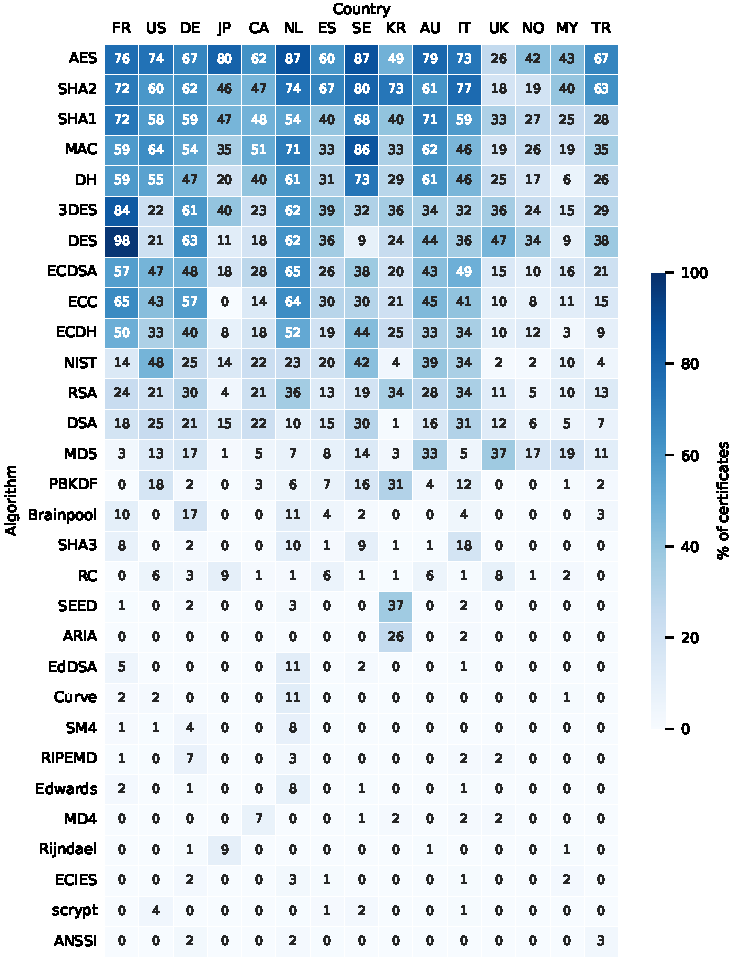
\includegraphics{cc_country_algorithm_heatmap}
  \caption{Share of CC certificates mentioning each algorithm, by scheme}
  \label{fig:cc-country-heatmap}
\end{figure}

\begin{figure}[htbp]
  \centering
  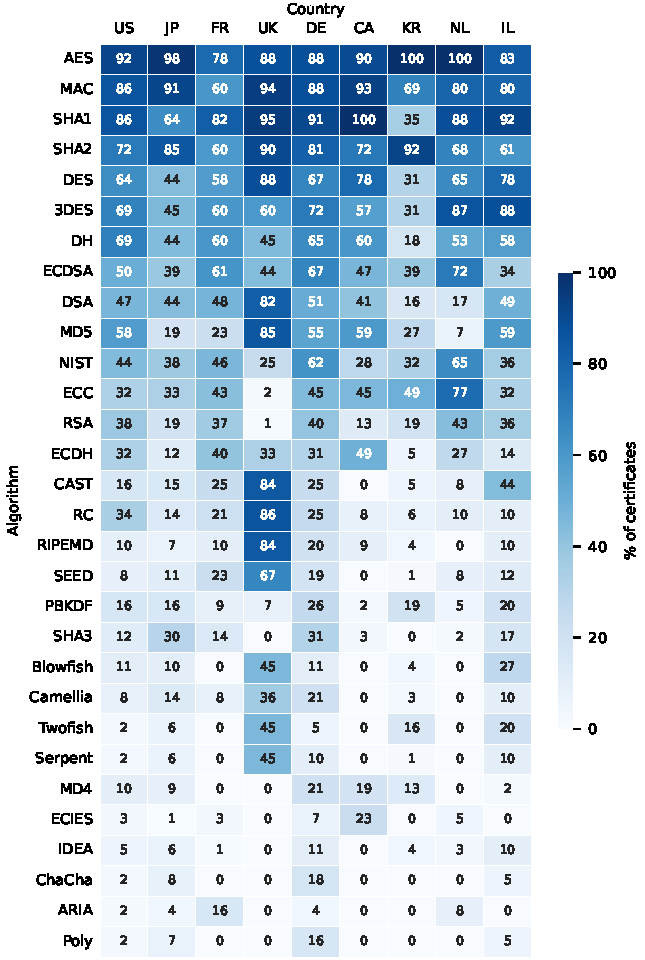
\includegraphics{fips_country_algorithm_heatmap}
  \caption{Share of FIPS~140 certificates mentioning each algorithm, by vendor
    country}
  \label{fig:fips-country-heatmap}
\end{figure}

\subsection{Product category and issue period}
\label{sec:results-country-confounders}

Two confounders affect the CC comparison. First, schemes certify different
product mixes: 89\,\% of French certificates are smart cards, while the largest
group of US certificates are network devices (34\,\%) and none are smart cards.
Figures~\ref{fig:cc-country-smartcards} and~\ref{fig:cc-country-network}
therefore compare the schemes within each of these two categories. Second,
schemes were active in different periods. UK certificates run from 1998 to 2017
with a median of 2006, while the median for the Netherlands is 2023.
Figures~\ref{fig:cc-country-older} and~\ref{fig:cc-country-recent} split the
certificates at 2017, the median issue year across the dataset.

The split separates the two effects. French DES mentions stay at 96--99\,\% in
both periods, so they follow from the smart-card product mix rather than from
the era. In contrast, US DES mentions drop from 34\,\% to 9\,\%. The low AES and
SHA-2 shares of the UK scheme are an era effect, because the UK appears only in
the earlier period. The Korean national ciphers are a current preference rather
than a legacy one: SEED rises from 32\,\% to 41\,\% and ARIA from 7\,\% to
44\,\% after 2017.

\begin{figure}[htbp]
  \centering
  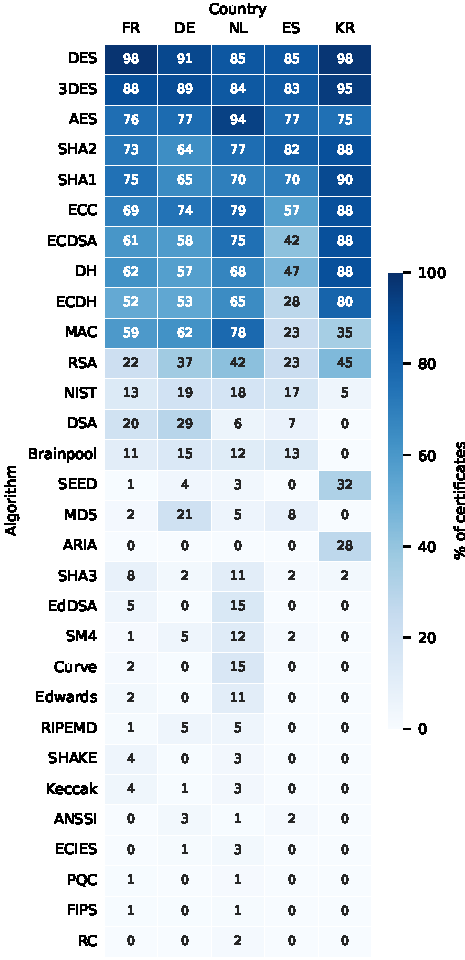
\includegraphics{cc_country_algorithm_heatmap_smartcards}
  \caption{Share of CC smart card certificates mentioning each algorithm, by
    scheme}
  \label{fig:cc-country-smartcards}
\end{figure}

\begin{figure}[htbp]
  \centering
  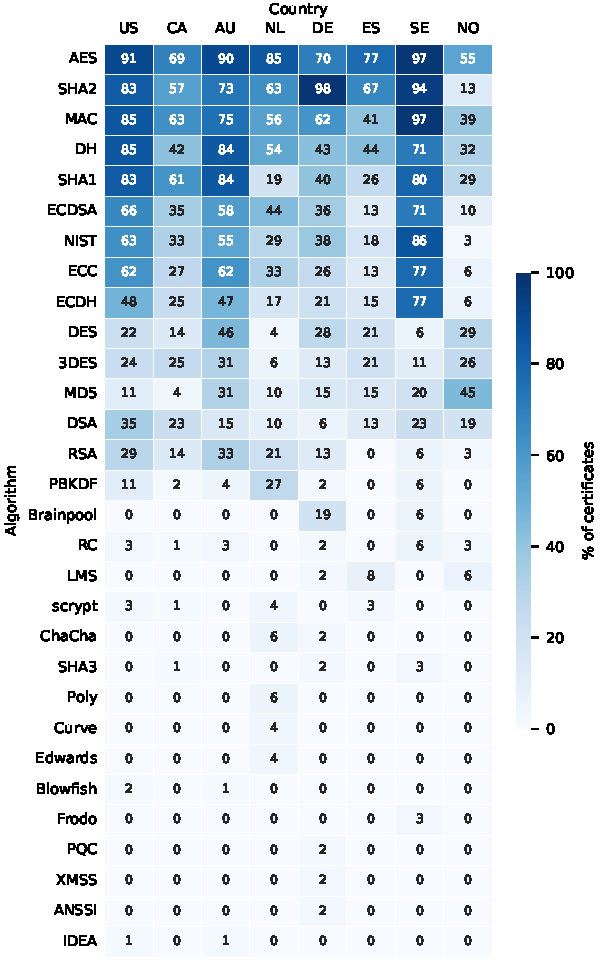
\includegraphics{cc_country_algorithm_heatmap_network}
  \caption{Share of CC network device certificates mentioning each algorithm,
    by scheme}
  \label{fig:cc-country-network}
\end{figure}

\begin{figure}[htbp]
  \centering
  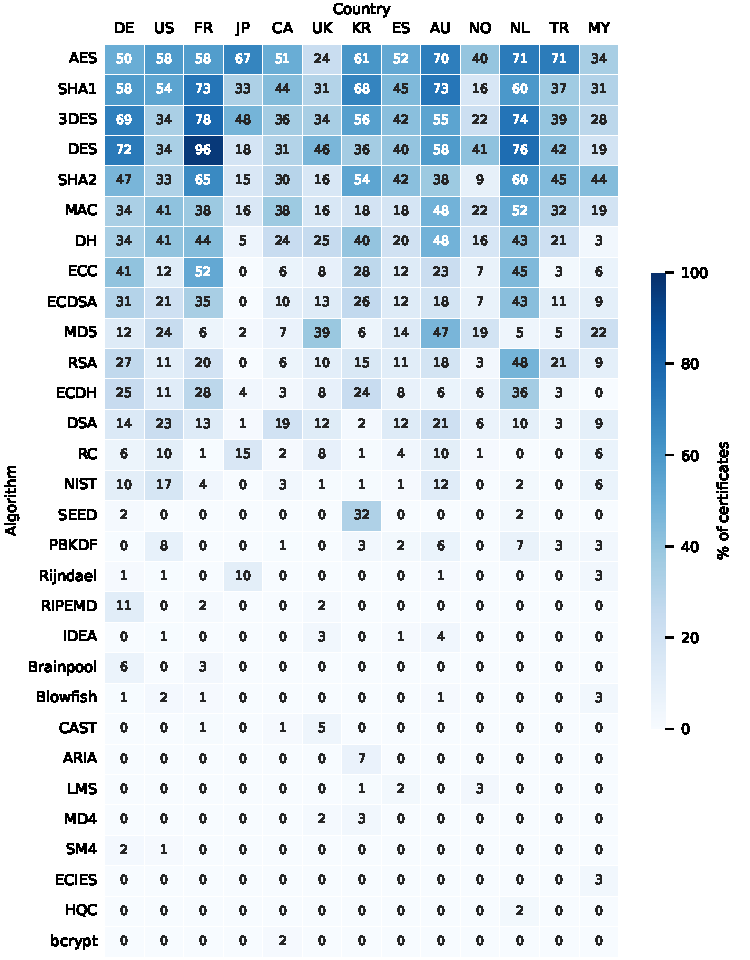
\includegraphics{cc_country_algorithm_heatmap_older}
  \caption{Share of CC certificates issued before 2017 mentioning each
    algorithm, by scheme}
  \label{fig:cc-country-older}
\end{figure}

\begin{figure}[htbp]
  \centering
  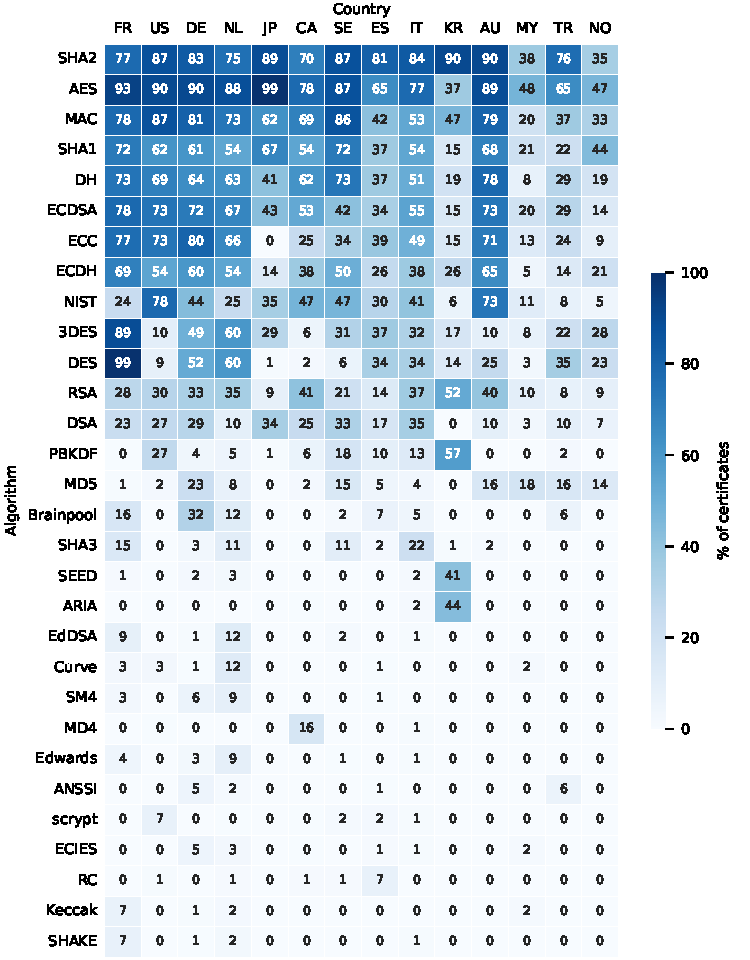
\includegraphics{cc_country_algorithm_heatmap_recent}
  \caption{Share of CC certificates issued in 2017 or later mentioning each
    algorithm, by scheme}
  \label{fig:cc-country-recent}
\end{figure}

\subsection{OpenSSL by country}
\label{sec:results-country-openssl}

A certificate counts as OpenSSL-based when OpenSSL appears among the crypto
libraries detected in its documents. This applies to 1,196 of 6,819 CC
certificates and 968 of 5,423 FIPS~140 certificates.
Figure~\ref{fig:openssl-country} shows how this share differs by country. Among
CC schemes it ranges from 53\,\% in Sweden to 1.4\,\% in France. Part of this
gap is product mix again, so the second panel restricts CC to network devices,
where Sweden reaches 83\,\% (this panel includes countries with at least 30
network device certificates). Among FIPS vendor countries, Germany (26\,\%) and
Japan (21\,\%) lead.

Figure~\ref{fig:openssl-gap} compares the algorithms mentioned by OpenSSL-based
certificates with those mentioned by other certificates. OpenSSL-based documents
tend to list the whole OpenSSL algorithm catalogue, so they mention almost every
algorithm more often. The elliptic-curve algorithms show the largest gap. ECDSA
and the NIST curves differ by about 40 percentage points in both schemes, and
ECDH does so among CC network devices, but only by 20 points in FIPS~140, where
DSA and Diffie--Hellman show larger gaps (about 33 points).
Among CC network devices, 3DES is the clearest exception: OpenSSL-based
certificates mention it 9 percentage points less often.

\begin{figure}[htbp]
  \centering
  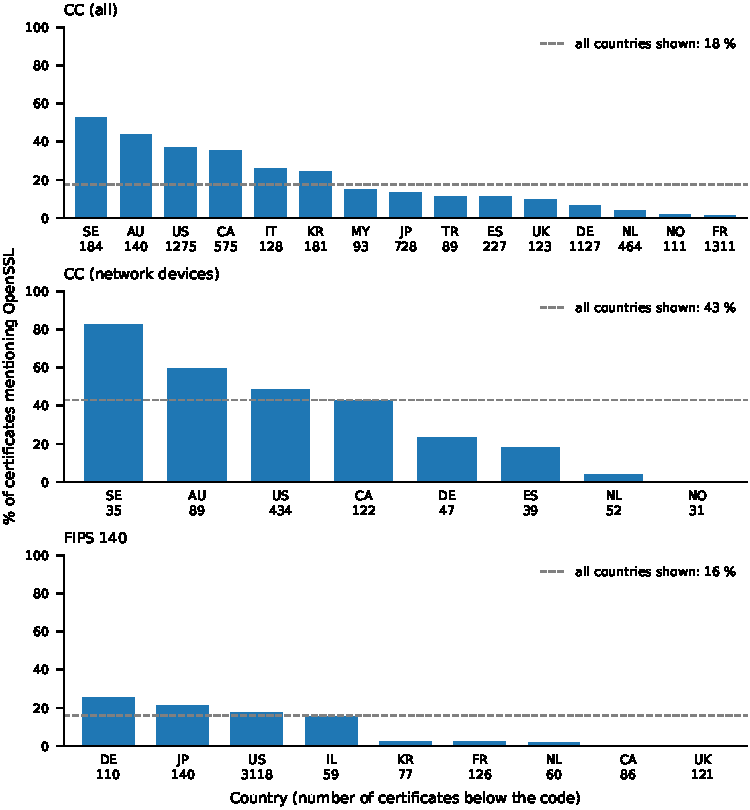
\includegraphics{openssl_share_by_country}
  \caption{Share of certificates mentioning OpenSSL, by country}
  \label{fig:openssl-country}
\end{figure}

\begin{figure}[htbp]
  \centering
  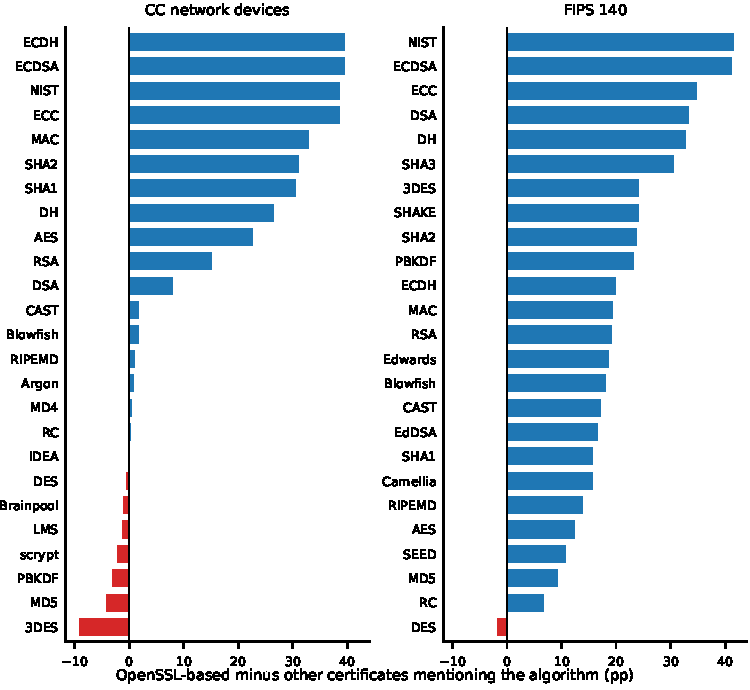
\includegraphics{openssl_algorithm_gap}
  \caption{Difference between the share of OpenSSL-based and other certificates
    mentioning each algorithm, for CC network devices and FIPS~140}
  \label{fig:openssl-gap}
\end{figure}

OpenSSL also ships several national ciphers: SEED and ARIA (Korea), Camellia
(Japan) and SM4 (China). Table~\ref{tab:national-ciphers} shows how often the
certificates that mention each cipher are OpenSSL-based, compared with all
certificates in the same scope. In FIPS~140, outside the home country, SEED,
ARIA, Camellia and SM4 mentions are OpenSSL-based about twice as often as the
baseline (26--38\,\% against about 16\,\%), so OpenSSL is a likely source of
these mentions. Korean CC certificates show the opposite: those mentioning SEED
or ARIA are less often OpenSSL-based than Korean certificates overall, which
suggests that Korean vendors use their own implementations. Groups with fewer
than ten certificates are too small to interpret. In the table, $n$ is the
number of certificates in the scope that mention the cipher, \enquote{OpenSSL}
is the percentage of them that are OpenSSL-based, and \enquote{Baseline} is the
percentage of all certificates in the scope that are OpenSSL-based.

\begin{table}[htbp]
  \centering
  \caption{OpenSSL-based certificates among those mentioning a national cipher}
  \label{tab:national-ciphers}
  \begin{tabular}{lllrrr}
    \toprule
    Scheme & Cipher (home) & Scope & $n$ & OpenSSL & Baseline \\
    \midrule
    CC   & SEED (KR)       & home      &  67 &  19.4 & 24.3 \\
    CC   & SEED (KR)       & elsewhere &  49 &   4.1 & 17.4 \\
    CC   & ARIA (KR)       & home      &  47 &  12.8 & 24.3 \\
    CC   & ARIA (KR)       & elsewhere &   4 & 100.0 & 17.4 \\
    CC   & Camellia (JP)   & elsewhere &   4 &   0.0 & 18.0 \\
    CC   & SM4 (CN)        & elsewhere & 111 &  18.9 & 17.5 \\
    CC   & GOST (RU)       & elsewhere &   1 &   0.0 & 17.5 \\
    \midrule
    FIPS & SEED (KR)       & home      &   1 &   0.0 &  2.6 \\
    FIPS & SEED (KR)       & elsewhere & 428 &  26.4 & 16.5 \\
    FIPS & ARIA (KR)       & elsewhere &  87 &  26.4 & 16.5 \\
    FIPS & Camellia (JP)   & home      &  19 &  63.2 & 21.4 \\
    FIPS & Camellia (JP)   & elsewhere & 331 &  36.0 & 16.0 \\
    FIPS & SM4 (CN)        & home      &   4 &   0.0 & 35.7 \\
    FIPS & SM4 (CN)        & elsewhere &  58 &  37.9 & 16.1 \\
    FIPS & GOST (RU)       & elsewhere &   7 &  14.3 & 16.2 \\
    \bottomrule
  \end{tabular}
\end{table}

\chapter{Discussion}
\label{ch:discussion}

\section{Interpretation of the findings}
\label{sec:interpretation}

{Write once the results exist. Answer each research question directly, then
explain what the findings mean for each audience: certification bodies, vendors,
buyers, and researchers who assess third-party cryptographic dependencies.}

A long certification lag is not automatically a security failure: a vendor may
backport fixes without changing the version string, and re-validating a module has
a real cost. The lag should therefore be read as a measure of the distance between
the certified and upstream states rather than as a direct measure of risk.

\section{Threats to validity}
\label{sec:threats}

\paragraph{Incomplete disclosure.} The largest threat is that the absence of a mention
does not imply the absence of a dependency, because vendors may redact or generalize
their dependency descriptions. All prevalence figures are therefore lower bounds on
actual use, and disclosure practices may differ between vendors, schemes, and
periods. An apparent trend may reflect changed disclosure rather than changed use.

\paragraph{A mention is not an evaluated dependency.} A library may appear in a document
without being evaluated, or without being within the certified boundary. The evidence
levels in Table~\ref{tab:evidence} mitigate this threat but do not remove it, since the
levels are based on what the documents state.

\paragraph{Extraction errors.} Text extraction from PDF documents can fail or corrupt
content, and both regular expressions and language models produce errors. Measuring
precision and recall on an annotated sample bounds these errors. The sample itself is
subject to annotator judgment and to sampling error.

\paragraph{Version semantics.} Version strings can hide backported patches, vendor builds,
or a validated provider that differs from the library using it, which affects the
lag defined in Equation~\ref{eq:lag}. The lag can also only be computed for certificates
with a stated version, and these may not represent all certificates.

\paragraph{Dataset dependence.} The analysis inherits any errors and coverage limits of
sec-certs. Pinning a snapshot makes the study reproducible, but the findings describe the
state of the data at that date.

\paragraph{Non-independent observations.} One vendor may hold many closely related
certificates, so raw certificate counts can overweight large product families. Results
should therefore also be reported per vendor or product family where this changes the
conclusion.

\section{Limitations}
\label{sec:limitations}

The study relies only on public documents. It does not inspect binaries or source code,
so no statement about a product's dependency is confirmed against the product itself.
It also does not assess the implementation quality of any library or whether a
particular product is vulnerable.

\chapter*{Conclusion}
\markright{\textsc{Conclusion}}
\addcontentsline{toc}{chapter}{Conclusion}

Summary of contributions and future work.


\printbibliography[heading=bibintoc]

\appendix
\chapter{Supplementary Material}
\label{app:supplementary}


\end{document}
